\documentclass[]{article}
%\usepackage{myart2e}
\usepackage{graphics}
\usepackage[dvips]{epsfig}
\usepackage[body={6.50in,9.00in},letterpaper,ignoreall,centering,headsep=1em,footskip=2.5em,marginparsep=.05in,marginparwidth=.8in]{geometry}
\usepackage{hyperref}
\usepackage{amssymb}
\usepackage{amsmath}
\usepackage{mathtools}
\usepackage{dsfont}
\usepackage{graphicx}
\usepackage{grffile}
\usepackage{epsfig}
\usepackage{makeidx}
\usepackage{multicol}
\usepackage{xspace}
\usepackage{algorithm}
%\usepackage{algorithmic}
\usepackage{algpseudocode}
\usepackage{textcomp}
%\usepackage{enumitem}
\usepackage{booktabs}
\usepackage{array}
\usepackage{url}
\usepackage{color}
\usepackage{ifpdf}
\usepackage{cite}
\usepackage{array}
\usepackage{enumitem}% http://ctan.org/pkg/enumitem
\usepackage{fancyvrb}

% declare the path(s) where your graphic files are
\graphicspath{{../img/}}
\DeclareGraphicsExtensions{.pdf,.png,.jpg,.eps}

%\setstretch{1.1}

\newcommand{\nc}{\newcommand}
% the Orion algo
\nc{\orion}{{\scshape Orion}\xspace}
% the orion program
\nc{\orionp}{{\tt orion}\xspace}

\def\ie{i.e.}
\def\lt{<}
\def\eg{e.g.}
\def\vec#1{{\mathbf{\boldsymbol #1}}}
\def\mat#1{\mathbf{#1}}
\def\tr{T}
\def\minspan{ \alpha}
\def\scost{ \beta}
\def\inputf{{\tt$<$fstem$>$}\xspace}


\renewcommand{\topfraction}{.95}
\renewcommand{\bottomfraction}{.95}


\hypersetup{
pdftitle={Orion 1.0.x Manual}, % title
pdfauthor={David C. Anastasiu and George Karypis},    % author
%bookmarks=true,                % show bookmarks bar?
colorlinks=true,               % false: boxed links; true: colored links
linkcolor=blue,                % color of internal links (change box color with linkbordercolor)
citecolor=blue,                % color of links to bibliography
filecolor=magenta,             % color of file links
urlcolor=red                   % color of % external links
}

% \setlength{\floatsep}{2pt}
% \setlength{\intextsep}{6pt}
% \setlength{\textfloatsep}{2pt}
% \setlength{\abovecaptionskip}{2pt}
% \setlength{\belowcaptionskip}{2pt}

\title{{\Huge \orion}\thanks{%
\orion is copyrighted by the regents of the University of Minnesota.
Related papers are available via WWW at URL: {\bf\sf
http://www.cs.umn.edu/\~{}dragos} }\\%
 {\LARGE A Software Package for Analysis of Resource Utilization Evolution}\\
 {\Large Version 1.0.0}}
\author{David C. Anastasiu and George Karypis \\ \\
	Department of Computer Science \& Engineering\\University of
Minnesota\\ Minneapolis, MN 55455 \\ \\ Contact email:
\href{mailto:dragos@cs.umn.com}{dragos@cs.umn.com} }
\date\today


\begin{document}
\maketitle
%\vspace{1in}
%\centerline{\huge DRAFT}
\clearpage

\tableofcontents
\clearpage



%*************************************************************************
\section{Introduction}
%*************************************************************************

Understanding how utilization of resources evolves over time is an important
task with diverse business applications. For example, an analysis of how PC
usage evolves over time can help provide the best overall user experience for
current customers, can help determine when they need brand new systems vs.
upgraded components, and can inform future product design to better anticipate
user needs.

As a way to understand usage evolution, consider application (resource) usage in
a computer or mobile device. The variables being observed may describe daily time
spent by a user interacting with a given application.
Figure~\ref{fig:usage-evolution} illustrates the idea of computer usage and its
evolution at a high level, grouping individual applications used by users into
categories, such as Productivity and Games, and representing usage in these
categories as vectors. A user's behavioral pattern may change over time. For
example, our hypothetical user has a decreased overall PC usage as time
progresses. Towards the end of the sequence, she spends more time surfing the
Web, and less time using productivity tools. Characterizing usage evolution of
many users enables us to find groups of users with similar trends (right-hand
side of Figure~\ref{fig:usage-evolution}), which may also benefit computer
hardware and software designers by providing design feedback and insight into upcoming
trends.

\begin{figure}[h] \centering
    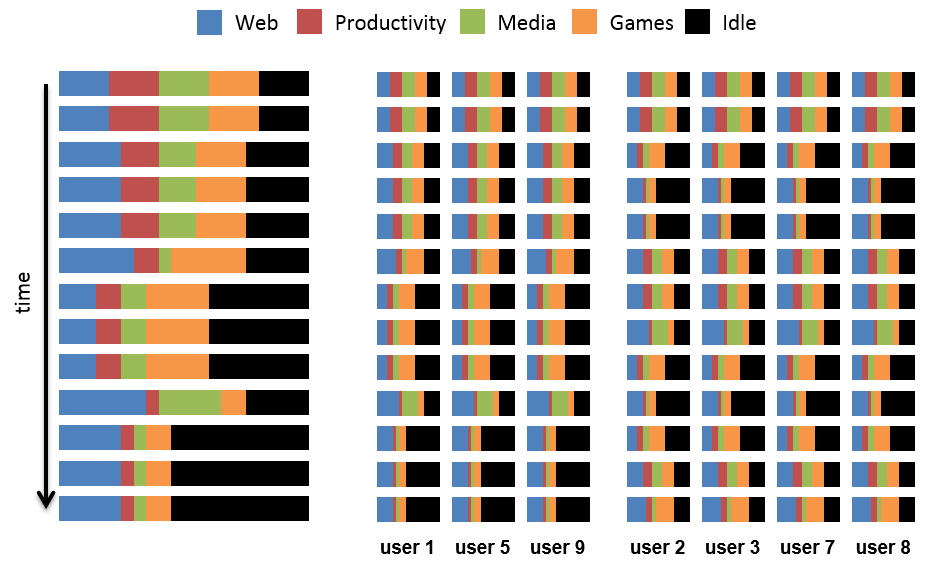
\includegraphics[width=0.7\columnwidth]{usage3}
    \caption{Computer usage evolution:  a user's sequence of PC usage vectors
    (on the left), and sequences of two similar sets of users (on the right).
    (Best viewed in color.)}
\label{fig:usage-evolution}
\end{figure}

%*************************************************************************
\section{Overview of \orion}
%*************************************************************************

\orion is a serial software package that facilitates evolution analysis of
multivariate resource utilization time series data, such as PC usage. \orion has
been developed at the Department of Computer Science \& Engineering at the
University of Minnesota and is freely distributed.
Its source code can be downloaded directly from {\em
http://www.cs.umn.edu/\~{}dragos/orion\/}.

\orion aims to characterize how a set of users utilize resources over time by
finding prototypical usage patterns (\emph{protos}) shared by users at different times
within their usage history. To do so, it models each user's usage evolution
as a sequence of protos and then performs a cross-user usage segmentation, i.e.,
a segmentation of the sequences of all users such that the error associated with
modeling each segment by one of the protos is minimized. The multivariate time
series segmentation problem has been previously addressed in the data mining
community (see~\cite{AbonyiFNA03, AbonyiFNA05, WangLY12, GuoLS14}), yet its goal has been
the optimal segmentation of a single time-series. Instead, \orion finds
the optimal segmentation of many time-series by a set of previously
unknown building blocks, which it learns during the search. The details of the
\orion algorithm can be found in~\cite{AnastasiuRTK15}.


%*************************************************************************
\section{The \orion program}
\label{sec:usage}
%*************************************************************************

\orion provides a stand-alone program that can be used to analyze multivariate
time-series resource utilization data. Additionally, several scripts enable
visualization of \orion's analysis output data. We describe first the format
of input data required by \orion, then \orion's execution, output, and
visualization scripts.

%=========================================================================
\subsection{Input file formats}
\label{sec:usage:iformat}
%=========================================================================

\orion expects as input \emph{sparse} multivariate time-series data.
Optionally, a file containing names/labels for each of the features in the
time-series data can be provided. The formats of these input files are described
in the following sections.

\subsubsection{Time series data}
\label{sec:usage:iformat:ts}

The primary input for \orion is sparse resource utilization time-series data for
a set of users. Each user's time-series is a sequence of sparse observation
vectors, each of which represents the user's multivariate resource utilization
in a time period (e.g., a week). Let the observation vectors of a user be stored
as the rows of a matrix, ordered in increasing time order. \orion's input
consists of a \emph{sparse matrix file} containing vertically concatenated
matrices for each of the user observation sequences, and a \emph{counts file},
which specifies the number of rows in the matrix file for each user sequence.

There may be gaps in a user's time series, as they may not be using
resources in every time period. These empty observation vectors should not be
included in their sequence. Additionally, a user's first observation vector may
not be in the same real time period as that of another user. \orion analyzes
relative usage changes/evolution. As such, while the order of vectors in each
user's time-series is important, the exact time periods when the observations
were made are not.

\orion accepts several ASCII and binary sparse matrix input file types. The
format of the input matrix file will be determined from the file's extension. In
the event the matrix format cannot be determined from the extension, \orion will
assume the input file is either in CSR or Cluto formats. Datasets stored in
binary formats usually take up less space and load faster during
execution. All binary formats assume little-endian encoding. The following
describes each of the acceptable sparse matrix file formats.
\begin{itemize}
  \item The \emph{CSR} ({\tt.csr} extension) and \emph{Cluto} ({\tt.clu})
  formats represent a sparse matrix row-wise in ASCII files, as {\tt<column-id,
  value>} pairs. Only the non-zero entries of the matrix are stored. Column ID
  numbering starts at 1. The Cluto format contains an additional header row with
  metadata information, three integers separated by space: the number of rows,
  the number of columns, and the number of non-zero values ($nnz$).

  \item The \emph{Triplet CSR} ({\tt.ijv}) format stores a sparse matrix in an
  ASCII file, containing a line for each value in the matrix, in the format ``\%d \%d
  \%f\textbackslash{}n'' (row id, column id, value).

  \item The \emph{Binary Row-wise CSR} ({\tt.binr}) format stores two 4-byte
  integers (number of rows and number of non-zero values), followed by 3 arrays.
  Let $n$ be the number of rows in the matrix and $nnz$ its number of non-zero
  values. The first array is a 4-byte integer pointer array ($ptr$) of length
  $n+1$ containing pointers into the next two arrays, the indicators ($ind$) and
  values ($val$) arrays. These pointers specify where each row starts, s.t. row
  $i$'s values are stored in the $val$ array starting at index $ptr[i]$ and
  ending at index $ptr[i+1]$. The indicators array $ind$ stores column IDs
  associated with values at the same index in the $val$ array. Needless to say,
  $ptr[0] = 0$ and $ptr[n] = nnz$. The $ind$ array is a 4-byte integer array of
  length $nnz$, and the val array is a 4-byte float array of length $nnz$.

  \item The \emph{Binary Triplet CSR} ({\tt.bijv}) format stores four 4-byte
  integers (number of rows, number of columns, $nnz$, and $writevals$).
  The variable $writevals$ is 1 if values are included and 0 otherwise. If
  values exist, the file then contains $nnz$ (row id, column id, value) triplets
  written as binary (int, int, float).   Otherwise, it contains $nnz$ (row id,
  column id) pairs written as binary (int, int).
\end{itemize}

The \emph{counts file} is an ASCII file, with as many lines as the number of
users/sequences, each line containing the observation count (sequence length) of
the associated user sequence, i.e., the number of row in the observation
sequence matrix, following the same user order as the input matrix.
By default, the counts file is assumed named {\tt$<$fstem$>$.counts}, where
{\tt$<$fstem$>$} is the name of the input matrix file. The parameter
\emph{-countsfile} allows specifying an alternate name.

\subsubsection{Feature labels}
\label{sec:usage:iformat:clabels}

Some of the analysis results that~\orion provides makes reference to features
in the data (e.g. applications whose utilization was observed) by name/label. If available,
feature labels can be provided in an ASCII file, one per line for each feature
in the data, in the order corresponding to the feature/column IDs in the input
matrix. By default, the labels file is assumed named {\tt$<$fstem$>$.clabels},
where \inputf is the name of the input matrix file. The parameter
\emph{-clabelsfile} allows specifying an alternate name for the feature
label file. In the event that the \emph{clabelsfile} file cannot be found,
labels will be automatically generated, in the format ``$l${\tt<fid>}'', where
{\tt<fid>} is the feature id.


%=========================================================================
\subsection{Using \orion}
\label{sec:usage:orion}
%=========================================================================

\orion is run via the \orionp executable. We start by listing its
runtime options, and then describe the analysis information it outputs.

\begin{tabbing}
{\sf\bf orion} \= [options] {\tt fstem} {\tt nprotos}
\end{tabbing}

\noindent
\begin{description}[align=left,style=nextline,leftmargin=*,font=\normalfont]

\item[{\bf\sf Description}]\mbox{}\\
   Orion performs multivariate resource utilization time series evolution analysis.

\item[{\bf\sf Parameters}]\mbox{}\\
  \vspace{-20pt} 
  \begin{itemize}[leftmargin=+.8in]
    \item[\bf fstem]
      The name of the file that contains the multivariate resource utilization
      time series data (Section~\ref{sec:usage:iformat:ts}).

    \item[\bf nprotos]
      The number of protos that should be used to encode the utilization sequences.
     
  \end{itemize}
  
  
\item[{\bf\sf Options}]\mbox{}\\
  \vspace{-20pt} 
  \begin{itemize}[leftmargin=+.8in]
    \item[\textbf{-rowmodel}=text]
       Specifies how the values will be scaled in each row.\\
       Possible values are:
  	   \vspace{-5pt} 
       \begin{itemize}[leftmargin=+.6in]
         \item[\tt none] No scaling.
         \item[\tt log]  Take the log of the raw values. [default]
         \item[\tt sqrt] Take the square-root of the raw values.
       \end{itemize}
       
    \item[\textbf{-colmodel}=text]
       Specifies how the values will be scaled in each column.\\
       Possible values are:
       \vspace{-5pt} 
       \begin{itemize}[leftmargin=+.6in]
         \item[\tt none] No scaling. [default]
         \item[\tt idf]  Scale by the inverse document frequency across all usage vectors.
         \item[\tt sidf] Scale by the inverse document frequency across sequences.
       \end{itemize}

    \item[\textbf{-minspan}=int]
       Specifies the minimum number of consecutive weeks that a proto must
       cover in a user's time-series.\\
       Default value is 5.

    \item[\textbf{-ncliters}=int]
       Specifies the maximum number of initial clustering iterations.\\
       Default value is 20.

    \item[\textbf{-niters}=int]
       Specifies the maximum number of segmentation refinement iterations.\\
       Default value is 20.

    \item[\textbf{-scost}=float]
       A per segment cost as a fraction of the error.\\
       Default value is .01.

    \item[\textbf{-mintp}=float]
       Specifies the minimum proto-to-proto transition probability to be
       analyzed.\\
       Default value is .20.

    \item[\textbf{-n2frac}=float]
       Specifies the maximum fraction of a vector to be analyzed for features.\\
       Default value is .80.

    \item[\textbf{-countsfile}=text]
       Required input file containing the number of rows in {\tt$<$fstem$>$} for
       each sequence.\\
       Default value is {\tt$<$fstem$>$.counts}.

    \item[\textbf{-clabelsfile}=text]
       Optional input file for the feature labels.\\
       Default value is {\tt$<$fstem$>$.clabels}. (labels will be generated if
       file does not exit).

    \item[\bf-writepaths]
       Outputs the proto paths of each sequence.

    \item[\textbf{-pathsfile}=text]
       Output file for the proto paths of each sequence.\\
       Default value is
       {\tt$<$fstem$>$.paths.c$<$scost$>$.s$<$minspan$>$.p$<$nprotos$>$}.

    \item[\bf-writeftrs]
       Outputs the key features for each proto. 

    \item[\textbf{-ftrsfile}=text]
       Output file for the key features for each proto.\\
       Default value is
       {\tt$<$fstem$>$.ftrs.c$<$scost$>$.s$<$minspan$>$.p$<$nprotos$>$}.

    \item[\bf-writep2pt]
       Outputs the global proto-to-proto transition probabilities.

    \item[\textbf{-p2ptfile}=text]
       Output file for the global proto-to-proto transition probabilities.\\
       Default value is
       {\tt$<$fstem$>$.p2pt.c$<$scost$>$.s$<$minspan$>$.p$<$nprotos$>$}.

    \item[\bf-writetrans]
       Outputs transition probabilities for a given transition level.

    \item[\textbf{-transfile}=text]
       Output file for the transition probabilities for a given transition level.\\
       Default value is
       {\tt$<$fstem$>$.trans.c$<$scost$>$.s$<$minspan$>$.p$<$nprotos$>$.l$<$translevel$>$}.

    \item[\textbf{-translevel}=int]
       Transition level to output transitions for. Must be $> 0$.\\
       Default value is 1.

    \item[\bf-writetinfo]
       Outputs frequent transitions and their key discriminative features.

    \item[\textbf{-tinfofile}=text]
       Output file for frequent transitions and their key discriminative features.\\
       Default value is
       {\tt$<$fstem$>$.tinfo.c$<$scost$>$.s$<$minspan$>$.p$<$nprotos$>$}.

    \item[\bf-writeprotos]
       Outputs the prototypical usage vectors.

    \item[\textbf{-protosfile}=text]
       Output file for the prototypical usage vectors.\\
       Default value is
       {\tt$<$fstem$>$.protos.c$<$scost$>$.s$<$minspan$>$.p$<$nprotos$>$}.

    \item[\textbf{-seed}=int]
       Specifies the seed for clustering.\\
       Default value is 1.

    \item[\textbf{-dbglvl}=int]
       Specifies the level of progress/debugging information to be displayed.\\
       Possible values are (2 and above can be combined in binary form):
  	   \vspace{-5pt} 
       \begin{itemize}[leftmargin=+.6in]
         \item[\tt 0] Disable all standard output.
         \item[\tt 1] Print general progress and output information. [default]
         \item[\tt 2] Include the protos.
         \item[\tt 4] Include per-sequence errors.
         \item[\tt 8] Include dynamic programming algorithm progress information.
       \end{itemize}

    \item[\bf-help]
       Displays the command-line options along with a description.

  \end{itemize}

\end{description}

\vspace{30pt}

With default \emph{-dbglvl} parameters, \orionp prints all analysis information
to {\tt stdout} and does not write any files. The \emph{-write*} and their
associated \emph{-*file} parameters can be used to store analysis details in
files. In the following, we describe \orionp program output under the default
debug level, \emph{-dbglvl=1}. Section~\ref{sec:usage:oformat} describes
possible output files for \orionp.

\subsubsection{Execution information}
\label{sec:usage:orion:exec}

\begin{figure}[h] 
\small
\begin{Verbatim}[frame=single]
orion -niters 3 -ncliters 5 seq1.csr 5 
Reading matrix seq1.csr...
Reading user sequence counts...
Generating feature labels...

-----------------
#seqs: 100, #vecs: 10010, #dims: 545, #protos: 5
rowmodel: log, colmodel: none, minspan: 5, niters: 3
scost: 0.010, mintp: 0.200, n2frac: 0.800

Initial clustering:
  iter:  0, totsqe: 1.4513e+03, nconsecutive:   5510/ 10010
  iter:  1, totsqe: 9.0365e+02, nconsecutive:   4883/ 10010
  iter:  2, totsqe: 8.8820e+02, nconsecutive:   4699/ 10010
  iter:  3, totsqe: 8.7484e+02, nconsecutive:   4598/ 10010
  iter:  4, totsqe: 8.7323e+02, nconsecutive:   4598/ 10010
\end{Verbatim}
\caption{Initial clustering output in \orionp}
\label{fig:verb:initclust}
\end{figure}

Figure~\ref{fig:verb:initclust} shows the beginning of the output produced by
\orionp. After displaying runtime parameters and some statistics on the input
data (\emph{\#seqs} - number of sequences/users, \emph{\#vecs} - number of
observation vectors across all sequences, \emph{\#dims} - number of features in
the observation vectors), \orionp displays execution statistics for the
$k$-means clustering iterations used to identify the initial protos. After each
iteration, \emph{totsqe} shows the sum of the square root error between the
observation vectors and their respective protos (the centers of the clusters
they are assigned to), and \emph{nconsecutive} shows the number of observation
vectors consecutively assigned to the same proto in the user sequences.

Execution in \orionp continues by displaying the proto-to-proto distance matrix
(see Section~\ref{sec:usage:orion:dist}) and the proto-to-proto transition
matrix (see Section~\ref{sec:usage:orion:p2pt}) for the initial protos. In the
second phase of the program, after encoding usage sequences with the identified
protos, \orionp employs an iterative process by which the protos are
automatically derived from the segmentation and an optimal segmentation is
determined from the protos using a dynamic programming algorithm. After each
iteration, the program displays the latest computed objective function value.
Additional details about the algorithms implemented in \orionp can be found
in~\cite{AnastasiuRTK15}. After the final protos and segmentations are computed,
\orionp displays analysis results, as described in
Sections~\ref{sec:usage:orion:dist}--\ref{sec:usage:orion:freqt}.

\subsubsection{Proto distances}
\label{sec:usage:orion:dist}

\begin{figure}[h] 
\small
\begin{Verbatim}[frame=single]
Proto distances -------------
 189.8 =>     0.0  400.7  179.3  295.1  297.3
 292.9 =>   400.7    0.0  298.6  410.1  432.8
  49.1 =>   179.3  298.6    0.0  177.4  179.1
 187.4 =>   295.1  410.1  177.4    0.0  295.8
 189.9 =>   297.3  432.8  179.1  295.8    0.0
End proto distances --------------
\end{Verbatim}
\caption{Proto distances matrix output in \orionp}
\label{fig:verb:dist}
\end{figure}

The proto distances output includes, for each proto, the proto intensity score,
followed by squared euclidean distances from the proto to each of the protos, in
ascending order of proto ID. Figure~\ref{fig:verb:dist} exemplifies output of a
proto distance matrix for 5 protos.

A proto is, in essence, the centroid of the set of resource utilization vectors
encoded by the proto after segmentation across all users, and is thus not
normalized. The proto intensity score is the squared $\ell^2$-norm of the proto
and measures the magnitude of the resource utilization values represented by the
proto.

Proto distance is an indicator of how similar two protos are. A large number of
small proto-to-proto distance values may be an indication that the requested
number of protos is too high.

\subsubsection{Proto-to-proto transition matrix}
\label{sec:usage:orion:p2pt}

\begin{figure}[h] 
\small
\begin{Verbatim}[frame=single]
Proto-to-proto transition matrix -------------
   19 =>  0.000 0.050 0.900 0.000 0.000
    9 =>  0.300 0.000 0.400 0.100 0.100
   19 =>  0.500 0.250 0.000 0.150 0.050
    2 =>  0.000 0.000 0.333 0.000 0.333
    3 =>  0.000 0.000 0.250 0.500 0.000
End proto-to-proto transition matrix -------------
\end{Verbatim}
\caption{Proto-to-proto transition matrix output in \orionp}
\label{fig:verb:p2pt}
\end{figure}

The proto-to-proto transition matrix includes global transition probability
values, computed over all transitions occurring in the proto sequences of all
users. Figure~\ref{fig:verb:p2pt} exemplifies output of a proto-to-proto
transition matrix for 5 protos. For each proto, \orionp outputs the number of
transitions from the proto to any other proto, followed by the probability
that usage transitions from that proto to each of the protos, sorted in
increasing proto ID order.

\vspace{10pt}

\subsubsection{Proto features}
\label{sec:usage:orion:ftrs}

\begin{figure}[h] 
\small
\begin{Verbatim}[frame=single]
Proto features -----
Proto: 0 [814 172.31 92.78]
  0.061 0.066 +0.024 0.061 l403
  0.046 0.060 +0.014 0.107 l185
  0.041 0.058 +0.011 0.149 l76
  0.039 0.005 +0.049 0.188 l363
...
Proto: 4 [54 147.79 77.96]
  0.222 0.065 +0.205 0.222 l294
  0.049 0.004 +0.065 0.271 l313
  0.042 0.004 +0.055 0.314 l347
...
  0.012 0.004 +0.011 0.806 l254
End proto features-----
\end{Verbatim}
\caption{Key proto features output in \orionp}
\label{fig:verb:ftrs}
\end{figure}

For each of the identified protos, \orionp shows analysis information for key
features, in the following format,\newline
\indent{\tt Proto: pid [pcount pint psqe]}\newline
\indent{\tt \quad fint$_1$ cint$_1$ fdis$_1$ sum$_1$ flabel$_1$}\newline 
\indent{\tt \quad fint$_2$ cint$_2$ fdis$_2$ sum$_2$ flabel$_2$}\newline 
\indent{\tt \quad $\ldots$ ,}\newline
%
which we further describe below. The list of features for each proto is sorted
in decreasing order of descriptive power/feature intensity ({\tt fint}). The
parameter \emph{-n2frac} determines the percent of features that are included in the
output for each proto. Figure~\ref{fig:verb:ftrs} gives an example of this type
of key feature output. Let $\vec p$ be a proto, and $p_j$ the value/weight of
the $j$-th feature within the proto. Furthermore, let $\vec c$ be the global
\emph{center}, the mean vector over all observation vectors in all user
sequences, and $c_j$ be similarly defined as $p_j$.
\begin{itemize}
  \item {\tt pid} is the integer Proto ID. Proto IDs start with 0.

  \item {\tt pcount} shows the number of observation vectors that were encoded by
  the proto, across all user sequences.

  \item {\tt pint} is the proto intensity score (see Section~\ref{sec:usage:orion:dist}).
  
  \item {\tt psqe} is the squared error between the proto and the center vector,
  $||\vec p - \vec c||_2^2$, and points to the discriminative power of the
  proto.

  \item {\tt fint} is the feature intensity score, measuring the descriptive power
  of the feature within the proto, computed as $p_j^2/||\vec p||_2^2$. 

  \item {\tt cint} is the associated feature intensity score in the center vector,
  measuring the global descriptive power of the feature across all vectors,
  computed as $c_j^2/||\vec c||_2^2$.

  \item {\tt fdis} is a measure of the discriminative power of the feature, computed
  as $(p_j - c_j)^2/||\vec p - \vec c||_2^2$. The added sign is an indicator
  whether $p_j > c_j\ (+)$, or not, $(-)$.

  \item {\tt sum} represents the cumulative feature intensity score for features
  displayed so far for the proto.

  \item {\tt flabel} is the feature label.

\end{itemize}


\subsubsection{Frequent proto-to-proto transitions}
\label{sec:usage:orion:freqt}

\begin{figure}[h] 
\small
\begin{Verbatim}[frame=single]
Frequent proto-to-proto transitions -------------
0 => 2 [18 0.900][172.31 44.67 110.74]
   -0.92 -2.509 0.038 0.001 0.05 l452
   -0.89 -2.225 0.039 0.002 0.10 l363
   -0.91 -2.443 0.034 0.001 0.14 l343
   -0.92 -2.501 0.033 0.001 0.18 l16
   -0.91 -2.364 0.033 0.001 0.23 l125
   -0.88 -2.133 0.034 0.002 0.27 l36
...
4 => 3 [2 0.500][147.79 171.60 85.01]
  +12.38 +2.555 0.000 0.065 0.11 l95
   +3.50 +1.491 0.004 0.074 0.20 l422
   -0.45 -0.597 0.222 0.058 0.28 l294
   +1.06 +0.717 0.033 0.121 0.34 l76
...
   -0.84 -1.833 0.014 0.000 0.80 l539
End frequent proto-to-proto transitions -------------
\end{Verbatim}
\caption{Frequent proto-to-proto transitions output in \orionp}
\label{fig:verb:freqt}
\end{figure}

The parameter \emph{-mintp} specifies the minimum proto-to-proto transition
probability to be analyzed. After computing probability values for all
proto-to-proto transitions, \orion displays, in decreasing transition
probability order, those proto transitions above the \emph{-mintp} cutoff. For
each transition, \orion displays some summary information about the protos
involved in the transition, followed by key feature information related to the
two protos. Figure~\ref{fig:verb:freqt} gives an example of this type
of key proto transitions output. Let $\vec p$ and $\vec q$ be the two protos in
a transition, s.t. usage transitions from $\vec p$ to $\vec q$, and let $p_j$
and $q_j$ be the value in the two protos for the $j$-th feature. The summary
information is in the following format,\newline
%%%%
\indent{\tt pid$_p$ => pid$_q$ [freq prob int$_p$ int$_q$, sqe]},\newline
which we further describe below. 
%%%%
\begin{itemize}
  \item {\tt pid$_p$} and {\tt pid$_q$} are the proto IDs for the protos transitioning
  from and to.

  \item {\tt freq} is the count of transitions from $\vec p$ to $\vec q$.

  \item {\tt prob} is the probability of transitioning from $\vec p$ to $\vec q$.

  \item {\tt int$_p$} and {\tt int$_q$} are the intensity scores of the two
  protos (see Section~\ref{sec:usage:orion:dist}).

  \item {\tt sqe} denotes the squared Euclidean distance between the two protos.

\end{itemize}

For each selected proto transition, \orion displays a number of statistics for
key features, in the format,
%%%
\indent{\tt \quad rdist logr fint$_p$ fint$_q$ dsum flabel,}\newline
%%%
which we further describe below. The first two numbers showcase the
differences between the feature utilization in the two protos, while the next
two show the respective feature magnitude in each of the two vectors. The list
of features for each proto transition is sorted in decreasing order of feature
discriminative power, $(p_j-q_j)^2 / ||\vec p - \vec q||_2^2$, where $j$ is the
ID of the chosen feature.
\begin{itemize}
  \item {\tt rdist} is the relative distance between the two feature values,
  computed as $|p_j - q_j|/p_j$. The added sign is an indicator
  whether $p_j \le q_j\ (+)$, or not, $(-)$.

  \item {\tt logr} is the log ratio between the two feature values,
  $\log(q_j/p_j)$.

  \item {\tt fint$_p$} and {\tt fint$_q$} are the feature intensity scores in
  the respective protos (see Section~\ref{sec:usage:orion:ftrs}).

  \item  {\tt dsum} is the cumulative discriminative power for features
  displayed so far for the proto transition.

  \item  {\tt flabel} is the feature label.
\end{itemize}

%=========================================================================
\subsection{Output file formats}
\label{sec:usage:oformat}
%=========================================================================

When invoked with certain parameters (see Section~\ref{sec:usage:orion}), \orion
can store a number of analysis results, which are described in the following
sections. All output files are ASCII text files.

\subsubsection{Proto paths}
\label{sec:usage:oformat:paths}

\orion encodes user sequences as sequences of protos, which can be stored in
the \emph{pathsfile} file. The proto sequences are stored one per line, in the
same order corresponding to the sequence matrices in the \inputf input file.
Each proto sequence is a list of proto IDs separated by space.

\subsubsection{Proto key features}
\label{sec:usage:oformat:ftrs}

For each of the identified protos, the \emph{ftrsfile} file stores key feature
information for the proto, in the format,\newline
\indent{\tt pid pcount pint psqe \textbackslash{}t{} fint$_1$ cint$_1$ 
fdis$_1$ sum$_1$ flabel$_1$ fint$_2$ cint$_2$ fdis$_2$ sum$_2$ flabel$_2$
$\ldots$}.\newline
The format components are described in detail in Section~\ref{sec:usage:orion:ftrs}.

\subsubsection{Proto-to-proto transitions}
\label{sec:usage:oformat:p2pt}

The \emph{p2ptfile} file stores the dense proto-to-proto global transition
probability matrix, computed over all transitions occurring in the proto
sequences of all users (see Section~\ref{sec:usage:orion:p2pt}). For each source
proto, in increasing proto id order, the file contains, on one line, the
probabilities that usage transitions from the source proto to the another
protos. Values in each line are separated by space and sorted in increasing
proto ID order.

\subsubsection{Level-wise proto transitions}
\label{sec:usage:oformat:trans}

Proto transitions can also be analyzed level-wise. Level $k$ transitions are
those transitions between the $k$-th proto and the $k+1$-th proto in a
proto-sequence. The \emph{transfile} file contains proto-to-proto transition
probabilities, counting only transitions in the requested level, in sparse
\emph{Triplet CSR} format. Each line of the file contains three values, in the
format, {\tt pid$_p$ pid$_q$ prob}, where {\tt pid$_p$} and {\tt pid$_q$} are
the proto IDs of the proto transitioning from and to, and {\tt prob} is the
probability of transitioning from $\vec p$ to $\vec q$. In addition,
\emph{start} (S) and \emph{end} (E) probabilities are included. A start
probability is stored as the triplet {\tt S pid$_p$ prob}, and represents the
probability of a sequence being encoded by proto $\vec p$ in level $k$. An end
probability is stored as the triplet {\tt pid$_p$ E prob}, and represents the
probability of a sequence not transitioning to level $k+1$. Level-wise
transition output can be graphically visualized using the {\tt transitions.py}
script (see Section~\ref{sec:usage:viz:trans}).

\subsubsection{Frequent proto-to-proto transitions}
\label{sec:usage:oformat:tinfo}

Frequent proto transitions and their key discriminative features are stored in
the \emph{tinfofile} file, in the format,\newline
%%%
\indent{\tt pid$_p$ pid$_q$ freq prob int$_p$ int$_q$ sqe \textbackslash{}t
rdist logr fint$_p$ fint$_q$ dsum flabel rdist logr \ldots}.\newline
%%%
For each included frequent transition, the initial 7 values describing the
protos involved in the transition are separated by a TAB character from the list
of sets of 6 feature characteristics of discriminating features for the
transition, separated by spaces. The format components are described in detail
in Section~\ref{sec:usage:orion:freqt}.

\subsubsection{Proto vectors}
\label{sec:usage:oformat:protos}

The \emph{protosfile} file stores the dense matrix whose columns are the protos,
sorted in increasing proto ID order. Each line in the file represents a
different feature and contains the proto values for the feature, separated by space. The
feature label is also included at the end of the line.


%=========================================================================
\subsection{Visualizing \orion output}
\label{sec:usage:viz}
%=========================================================================

Some of the \orionp output files can be used to create visualizations depicting
proto transitions and/or evolutions. The following sections describe
two Python scripts included in the \orion distribution for this purpose.

\subsubsection{The sankey.py script}
\label{sec:usage:viz:sankey} 

% \usepackage{graphics} is needed for \includegraphics
\begin{figure}[htp]
\begin{center}
  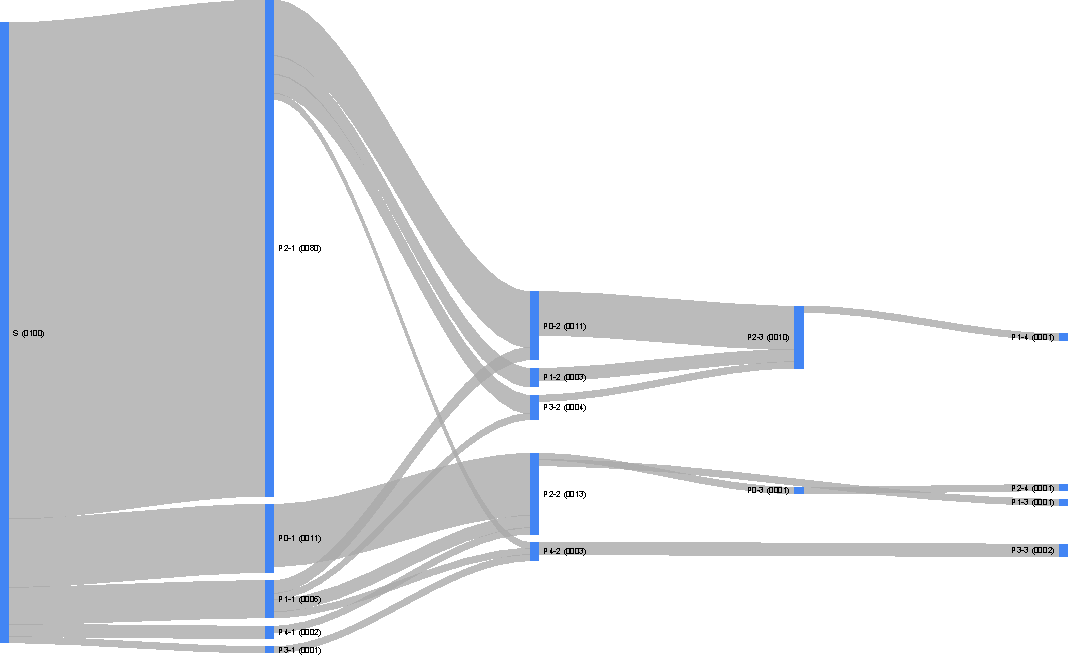
\includegraphics[width=0.9\columnwidth]{sankey}
  \caption{Proto evolution. Each (blue) vertical line represents a
behavior state, either \emph{Start} ($S$) or one of the $p$ protos, and its
extent is proportional to the proto level frequency. Curve (gray) lines show
users transitioning from state to state. Proto states are labeled with their ID,
level in sequence, and their frequency, i.e., the number of users that have that
proto at that level in their proto sequences.}
  \label{fig:sankey}
\end{center}
\end{figure}

The {\tt sankey.py} script creates a Sankey diagram depicting proto transitions
up to a given number of levels. Figure~\ref{fig:sankey} gives an example of a
diagram created using the script. The script requires the \emph{pathsfile}
\orionp output file as input to create a proto evolution chart (see
Section~\ref{sec:usage:oformat:paths}). Optionally, when invoked with the
\emph{-{}-mode proto} or \emph{-{}-mode rproto} parameters, it can create proto
Sankey evolution diagrams for each proto. In these modes, the script also
requires the \emph{ftrsfile} \orion output file (see
Section~\ref{sec:usage:oformat:ftrs}), and uses the information therein to
create pie charts displaying feature importance in each proto.

The output generated by the {\tt sankey.py} script is an {\tt html} file. The
output Web page uses the JavaScript package {\tt google.visualization.Sankey}
from Google
Charts\footnote{\href{https://developers.google.com/chart/}{https://developers.google.com/chart/}}
to create an interactive Sankey chart. When hovering over each transition edge
in the chart, all others will be partially faded. Figure~\ref{fig:verb:sankey}
shows usage information for the {\tt sankey.py} script.


\begin{figure}[h]
\small
\begin{Verbatim}[frame=single]
usage: sankey.py [-h] [-f MINFREQ] [-l MAXLEVEL] [-m MODE]
                 pathsfile [ftrsfile]

positional arguments:
  pathsfile             File containing the proto paths of each sequence.
  ftrsfile              File containing the key features for each proto 
                             (required for modes proto and rproto).

optional arguments:
  -h, --help            show this help message and exit
  -f MINFREQ, --minfreq MINFREQ
                        Minimum frequency to include a transition in the chart.
  -l MAXLEVEL, --maxlevel MAXLEVEL
                        Maximum number of levels to show in the chart (for mode global).
  -m MODE, --mode MODE  Type of chart to show:
                            global  Show global evolution chart [default]
                            proto   Show per-proto evolution
                            rproto  Show reverse per-proto evolution
\end{Verbatim}
\caption{Usage information for the sankey.py script}
\label{fig:verb:sankey}
\end{figure}

\subsubsection{The transitions.py script}
\label{sec:usage:viz:trans}

\begin{figure}[h] \centering
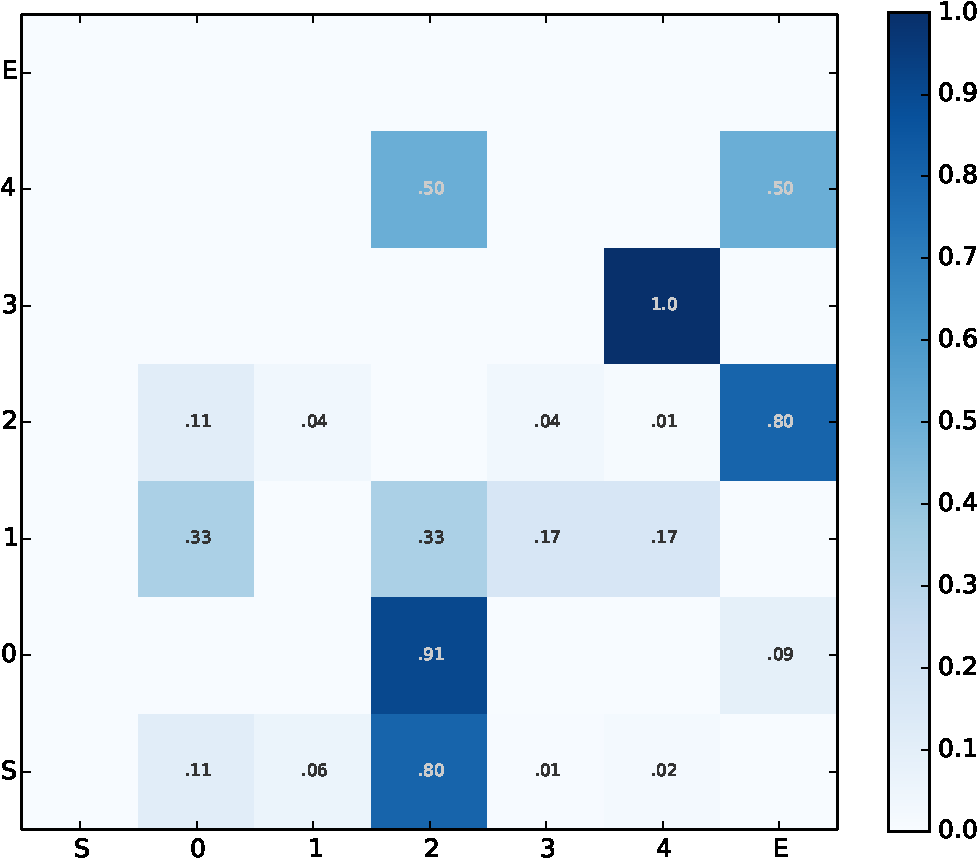
\includegraphics[width=0.4\columnwidth]{tprob}
\caption{Proto level-1 transitions. $S$ and $E$ are the \emph{Start} and \emph{End}
states, and the numbers denote protos. Each row shows the probabilities of a
user transitioning from the proto identified by the row ID towards other protos,
identified by column IDs. We only show probabilities above $0.01$ in the
transition matrix. }
\label{fig:proto-transitions}
\end{figure}

The {\tt transitions.py} script depicts level-wise proto transitions stored
in the \emph{transfile} \orionp output file (see
Section~\ref{sec:usage:oformat:trans}). Figure~\ref{fig:proto-transitions}
gives an example of its output. The script requires the \emph{pyplot} package
and, by default, creates a figure that is interactively displayed. Optionally,
the figure can be stored in a file compatible with \emph{pyplot} file storage
options (e.g., {\tt png}, {\tt eps}, {\tt pdf}, etc.), and the interactive
figure can pe disabled. Figure~\ref{fig:verb:transitions} shows usage
information for the {\tt transitions.py} script.

\begin{figure}[h]
\small
\begin{Verbatim}[frame=single]
usage: transitions.py [-h] [-ns] [-t TITLE] [-o OFILE] [-m MINP] transfile

positional arguments:
  transfile             File containing transition probabilities for a given
                        transition level.

optional arguments:
  -h, --help            show this help message and exit
  -ns, --noshow         Do not display the figure.
  -t TITLE, --title TITLE
                        Chart title.
  -o OFILE, --ofile OFILE
                        Output file for the chart (must have an accepted
                        pyplot output format extension).
  -m MINP, --minp MINP  Minimum transition probability to display text for.
\end{Verbatim}
\caption{Usage information for the transitions.py script}
\label{fig:verb:transitions}
\end{figure}


\subsection{Execution examples}
\label{sec:usage:exec}

In this Section, we include some examples of usage evolution analysis with
\orionp and its included visualization scripts. The distribution includes an
example time series input file, in the {\tt data} directory, named {\tt
seq1.csr}, and its associated counts file, {\tt seq1.csr.counts}. An example
feature labels file that does not conform to the default naming convention for
a \emph{clabelsfile} is also included. The included data are randomly generated
based on real PC application usage data described in~\cite{AnastasiuRTK15}. The
examples below will use these data files.

\begin{itemize}
  \item Execute an \orionp analysis, requesting 5 prototypical usage
  vectors, and print results to {\tt stdout}.\newline
  %% 
  \verb| ~$ orion data/seq1.csr 5|
  %%
  \item Provide a custom feature labels file for the previous analysis.\newline
  %% 
  \verb| ~$ orion data/seq1.csr 5 -clabelsfile data/seq1.labels|
  %%
  \item Specify a smaller segment generation cost and fewer segmentation
  refinement iterations.\newline
  %% 
  \verb| ~$ orion data/seq1.csr 5 -scost 0.005 -niters 10|
  %%
  \item Store resulting prototypical usage vectors using the default
  \emph{protosfile} file name and suppress {\tt stdout} output.\newline
  %% 
  \verb| ~$ orion data/seq1.csr 5 -writeprotos -dbglvl 0|
  %%
  \item Store level-1 proto transition probabilities in a custom file,
  and use it to generate a transition probability visualization
  chart.\newline
  %% 
  \verb| ~$ orion data/seq1.csr 5 -writetrans -transfile data/seq1.trans|\newline
  %% 
  \verb| ~$ scripts/transitions.py data/seq1.trans|
  %%
  \item Store the transitions chart in a {\tt pdf} file, preventing the
  display of the interactive chart.\newline
  %% 
  \verb| ~$ scripts/transitions.py data/seq1.trans -o data/seq1.trans.pdf -ns|
  %%
  \item Execute an \orionp analysis, requesting 5 prototypical usage
  vectors, and store the \emph{pathsfile} and \emph{ftrsfile} output files
  using their default names.\newline
  %% 
  \verb| ~$ orion data/seq1.csr 5 -writepaths -writeftrs|
  %%
  \item Use the \emph{pathsfile} to generate an usage evolution Sankey
  diagram, limited to the first 3 transition levels.\newline
  %% 
  \verb| ~$ scripts/sankey.py data/seq1.csr.paths.c0.010.s5.p5 -l 3 > data/sankey.html|
  %% 
  \item Use the \emph{pathsfile} and \emph{ftrsfile} files to generate Sankey
  evolution diagrams for each proto.\newline
  %% 
  \verb| ~$ scripts/sankey.py data/seq1.csr.paths.c0.010.s5.p5 data/seq1.csr.ftrs.c0.010.s5.p5|
  \verb|    -m proto > data/sankey2.html|
  %% 
\end{itemize}



%*************************************************************************
\section{System requirements and contact information}
\label{sec:epilogue}
%*************************************************************************

\orion is written entirely in ANSI~C, and is portable on most Unix systems
that have an ANSI~C compiler (the GNU~C compiler will do). It has been
tested on Linux and OSX. Instructions on how to build and install
\orion can be found in the files {\tt BUILD.txt} or {\tt BUILD-Windows.txt} of
the distribution.

\orion has been extensively tested on a number of different architectures.
However, even though \orion contains no known bugs, this does not mean that all
of its bugs have been found and fixed. If you have any problems, please send email to
\href{mailto:dragos@cs.umn.edu}{dragos@cs.umn.edu} with a brief description of
the problem. Also, any future updates to \orion will be made available on WWW at
\href{http://www.cs.umn.edu/~dragos/orion}{http://www.cs.umn.edu/\~{}dragos/orion\/}.

%******************************************************************************
\section{Copyright \& license notice}
\label{sec:license}
%******************************************************************************

\orion is copyrighted by the Regents of the University of Minnesota. 
It is licensed under the MIT License;
you may not use this program except in compliance with the License.
You may obtain a copy of the License at: 
\href{http://opensource.org/licenses/MIT}{http://opensource.org/licenses/MIT}.

Unless required by applicable law or agreed to in writing, software
distributed under the License is distributed on an "AS IS" BASIS,
WITHOUT WARRANTIES OR CONDITIONS OF ANY KIND, either express or
implied. See the License for the specific language governing
permissions and limitations under the License.



\clearpage
%*************************************************************************
{
\bibliographystyle{plain}
\bibliography{orion}
}

\end{document}
